%%%%%%%%%%%%%%%%%%%%%%%%%%%%%%%%%%%%%%%%%%%%%%%%%%%%%%%%%%%%%%%%%%%%%%
% How to use writeLaTeX:
%
% You edit the source code here on the left, and the preview on the
% right shows you the result within a few seconds.
%
% Bookmark this page and share the URL with your co-authors. They can
% edit at the same time!
%
% You can upload figures, bibliographies, custom classes and
% styles using the files menu.
%
%%%%%%%%%%%%%%%%%%%%%%%%%%%%%%%%%%%%%%%%%%%%%%%%%%%%%%%%%%%%%%%%%%%%%%

\documentclass[12pt]{article}

\usepackage{sbc-template}

\usepackage{graphicx,url}

%\usepackage[brazil]{babel}
\usepackage[utf8]{inputenc}


\sloppy

\title{Implantação contínua: Implantação ágil no desenvolvimento de software}

\author{Thiago  de Souza Fonseca Ribeiro\inst{1}}


\address{UnB -- Universidade de Brasília -- Campus Gama -- FGA
  \email{thiagovsk@aluno.unb.br}
}

\begin{document}

\maketitle

\begin{abstract}
  This meta-paper describes the style to be used in articles and short papers
  for SBC conferences. For papers in English, you should add just an abstract
  while for the papers in Portuguese, we also ask for an abstract in
  Portuguese (``resumo''). In both cases, abstracts should not have more than
  10 lines and must be in the first page of the paper.
\end{abstract}

\begin{resumo}
  Este meta-artigo descreve o estilo a ser usado na confecção de artigos e
  resumos de artigos para publicação nos anais das conferências organizadas
  pela SBC. É solicitada a escrita de resumo e abstract apenas para os artigos
  escritos em português. Artigos em inglês deverão apresentar apenas abstract.
  Nos dois casos, o autor deve tomar cuidado para que o resumo (e o abstract)
  não ultrapassem 10 linhas cada, sendo que ambos devem estar na primeira
  página do artigos.
\end{resumo}

\section{Introdução}\label{sec1}

\section{Outro Capitulo} \label{sec2}

\section{Metodologia: Planejamento da Revisão Sistemática} \label{sec3}

Segundo Kitchenham \cite{kitchenham2004procedures} a maior parte das pesquisas começa com uma revisão de literatura, no entanto, para ter valor científico é necessário que essa revisão seja feita de forma abrangente, não tendenciosa, aberta e objetiva. Por isso a necessidade de utilizar a revisão sistemática, que deve identificar, interpretar e avaliar todas as pesquisas disponíveis e relevantes sobre uma questão \cite{keele2007guidelines}. Para isso a revisão sistemática segue um protocolo de busca, que deve conter todas as informações que permitam que a revisão seja repetida por outros pesquisadores interessados no trabalho desenvolvido.

De acordo com \cite{brereton2007lessons} a revisão sistemática envolve três fases, resumidamente as fases são: Planejamento, Execução e análise dos resultados. Neste trabalho cada faze aborda:

 \begin{itemize}
   \item  \textbf{Planejamento: } Identificação  das  necessidades  para  a  revisão  e  elaboração do protocolo, o protocolo que deverá orientar toda a revisão sistemática. Nele deve conter as informações sobre o objetivo, a descrição do problema, as questões
da pesquisa e os métodos e critérios utilizados para a busca, seleção, avaliação e extração de dados.
   \item  \textbf{Execução: } Na fase de execução, os métodos descritos no protocolo são aplicados e documentados, além da identificação da pesquisa, seleção e avaliação da qualidade  dos  estudos.
      \item  \textbf{Análise dos Resultados: }Na fase de análise dos resultados os dados dos estudos são extraídos e sintetizados e os
resultados são analisados.
 \end{itemize}

\subsection{Objetivos} \label{sec3:subsec1}

O objetivo deste trabalho foi identificar como é feito o processo de implantção de software em equipes de desenvolvimento que utilizam métodos ágeis, identificando quais os procedimentos e técnicas utilizadas nos trabalhos relacionados, a partir de publicações científicas ou estudos primários.

\subsection{Questão de Pesquisa} \label{sec3:subsec2}

A partir do objetivo estabelecido na Seção \ref{sec3:subsec1}, foi elaborada a seguinte questão de pesquisa:

 \begin{itemize}
   \item  \textbf{Questão de Pesquisa: Quais são as formas de otimizar o processo de implantação de software utilizadas em equipes que trabalham utilizando métodos ágeis? }
 \end{itemize}

Essas questões deverão ser respondidas ao final da revisão sistemática.

\subsection{Métodos de Busca de Publicações} \label{sec3:subsec3}

Esta  Subseção  descreve  onde  e  como  foram  realizadas
as  buscas  desta  pesquisa. Apresentam-se também as palavras-chave utilizadas para a geração da string  de busca e os idiomas aceitos para a seleção dos resultados.

As fontes selecionadas para realização deste trabalho foram pesquisadas nas bases eletrônicas de dados disponíveis no portal CAPES, incluindo documentos indexados nas seguintes bases:

 \begin{itemize}
   \item  \textbf{Periódicos CAPES}
   \item  \textbf{IEEEXplore}
   \item  \textbf{Springer}
 \end{itemize}

As seguintes palavras foram utilizadas para fazer as buscas de estudos:

 \begin{itemize}
   \item  \textbf{Agile}
   \item  \textbf{Process Software Deployment}
   \item  \textbf{Devops}
   \item  \textbf{Continuous Delivery}
   \item  \textbf{Continuous Deploy}

 \end{itemize}

Com o intuito de abordar as palavras chave anteriormente definidas, foram definidas as seguitnes strings de busca:

 \begin{itemize}
   \item  \textbf{("deploy" OR "deployment") AND  "agile" AND "software" AND ("devops" OR "continuous delivery" OR "continuous deploy") }
 \end{itemize}

É importante ressaltar que a strings de busca deverá na medida do possível ser igual em todas as máquinas de busca, contudo poderá existir adaptações mas levando em consideração que a string adaptada deverá ser logicamente equivalente a string original.

O idioma escolhido foi o Inglês, também considerou-se qualquer tipo de trabalho ou artigo que fizesse abordagem sobre características de implantação de software no contexto de métodos ágeis.

\subsection{Critérios de Seleção} \label{sec3:subsec4}

Após a realização das buscas, serão incluídos na revisão todos os artigos encontrados com a utilização do método descrito na subseção \ref{sec3:subsec5} que satisfaçam todos os seguintes critérios de inclusão:

 \begin{itemize}
   \item  \textbf{Critério de inclusão:} O resultado deve estar no indoma inglês.
   \item  \textbf{Critério de inclusão:} O resultado deve estar disponível integralmente.
   \item  \textbf{Critério de inclusão:} O resultado deve conter no título, ou resumo, ou conclusão,  informações relevantes sobre o tema desse trabalho.
 \end{itemize}

 Após a realização das buscas, serão excluídos na revisão todos os artigos que satisfaçam todos os seguintes critérios de inclusão:

 \begin{itemize}
   \item  \textbf{Critério de exclusão:} O resultado não trata do contexto de implantação e desenvolvimento de software.
 \end{itemize}

Para avaliar a qualidade dods estudos foi levado em consideraçãoos seguintes aspectos:

 \begin{itemize}
   \item  \textbf{O trabalho deve ser interessante para o estudo} Esse aspecto condiz com a idéia de que os trabalhos encontrados devem estar de acordo com trabalhos conhecidos ou em publicações de artigos bem avaliados pelo qualis da CAPES.
   \item  \textbf{O trabalho deve conter evidências importantes para a pesquisa} É importante que o trabalho encontrado tenha evidências que possam ajudar na revisão sistemática, trabalhos que forem encontrados dentro da pesquisa pela string de busca mas que não condizem com o escopo do trabalho serão descartdos.
 \end{itemize}

\subsection{Procedimentos Para Extração de Dados} \label{sec3:subsec5}

Foi realizado uma busca em inglês em cada uma das fontes definidas na seção \ref{sec3:subsec3}, utilizando as strings de busca definidas na seção \ref{sec3:subsec3}, a partir da busca foram lidos todos os títulos, ou resumos, ou conclusões dos artigos encontrados. Isso foi necessário para saber quantos passaram pelos critérios de inclusão e quais não foram de acordo com os critérios de exclusão, citados na seção \ref{sec3:subsec4}, ou seja, aqueles trabalhos que os resultado não continham relevância no título, ou resumo, ou conclusão foram exluídos.

\subsection{Extração de Resultados} \label{sec3:subsec6}

Após  esta leitura inicial ,  os  resultados que foram incluídos a partir dos critérios de inclusão foram  selecionados  para  serem  lidos e  analisados de forma integral, assim os resultados aprovados pelos critéios de inclusão serão considerados neste estudo.

\section{Execução da Revisão Sistemática} \label{sec4}

Para a execução da revisão sistemática foram realizados diversas consultas a base dados entre o período de  8/10/2015 a 8/11/2015 com as diferentes strings de busca citadas na seção \ref{sec3:subsec2} foram realizadas duas iterações para identificar os trabalhos relacionados de acordo com os critérios definidos na seção \ref{sec3:subsec4}.

\subsection{Execução das Buscas} \label{sec4:subsec1}

Dado a quantidade de palavras chave, foi nessesário testar algumas combinações possíveis para montar as strings de busca, foram levantadas algumas strings de busca iniciais que não foram suficientes como: "agile process software deployment" que trazia várias abordagens que não seriam interessantes para este trabalho, com isso foram montadas operações boleanas com AND e OR para filtrar melhor os trabalhos relacionados. Outra evolução da string de busca foi de acordo com a percepção de outros termos que são utilizados nos trabalhos sobre métodos ágeis que são por exemplo : Devops, Continuous Integration, Continuous Delivery e Continuous Deploy, esse aprendizado serviu para refinar a string de busca, também percebeu-se que a palavra "process" anteriormente inserida como um AND na busca diminuia a quantidade de resultados relevantes.

\subsection{Seleção Preliminar} \label{sec4:subsec2}
Após o refinamento das strings de busca, foram realizadas as buscas de acordo com as bases definidas na seção \ref{sec3:subsec3}, algumas ferramentas dificultavam o uso da string de busca, como solução paliativa a ação tomada foi quebrar a string de busca nas operações OR e AND para conseguir um resultado melhor. Os seguintes resultados foram obtidos:

 \begin{itemize}
   \item  \textbf{Periódicos CAPES:} Foram encontrados ao total 58 artigos, para refinar a busca dos periódicos encontrados na base foram removidos da busca os seguintes resultados: Activities , Comprehension, Self, Domains, Communications, Environments, Improvement. Neste primeiro momento também não foram removidos os artigos duplicados na busca.
   \item  \textbf{IEEE explorer:} Utilizando a string de busca foram encontrados 62 artigos, sem remover artigos duplicados.
   \item  \textbf{Springer:} Foram encontrados 169 artigos, aplicando os seguintes filtros: English, Computer Science, SWE and Article. Para diminuir a quantidade de artigos para serem analisados, também foi feito um filtro de datas, aplicando do ano de 2010 até o ano de 2015, e a quantidade final encontrada foi de 110 artigos.
   \item  \textbf{Google Schoolar:} Vários resultados foram encontrados nessa busca, porém essa base será utilizada como base complementar.
 \end{itemize}

\subsection{Seleção Final} \label{sec4:subsec3}

Pelo tempo disponível para o desenvolvimento do trabalho, deu-se a necessidade de filtrar os artigos por data, ou seja, os mais novos foram vistos primeiro. No caso da grande quantidade encontrada em todas as bases e dado o tempo para o desenvolvimento do trabalho a primeira filtragem foi feita pelo título e pela própria descrição do artigo encontrado na busca.

Após essa filtragem inicial os artigos escolhidos passaram pelos critérios definidos na seção \ref{sec3:subsec4}, tendo como análise seus títulos, resumos, introduções e conclusões, as discussões sobre os resultados obtidos nesta fase estão descritos na seção \ref{sec5}, além disso também foram removidos os artigos duplicados, totalizando :

\begin{itemize}
  \item \textbf{CAPES:} 3 artigos
    \item \textbf{IEEE:} 12 artigos
    \item \textbf{SPRINGER:} 2 artigos
\end{itemize}

\section{Análise dos resultados} \label{sec5}

Nesta  seção,  as  publicações  selecionadas  foram  analisadas  levando  em  consideração  o
objetivo deste trabalho, buscando responder as questão de pesquisa definida


\section{Conclusão} \label{sec6}

\begin{table}[ht]
\centering
\caption{Variables to be considered on the evaluation of interaction
  techniques}
\label{tab:exTable1}
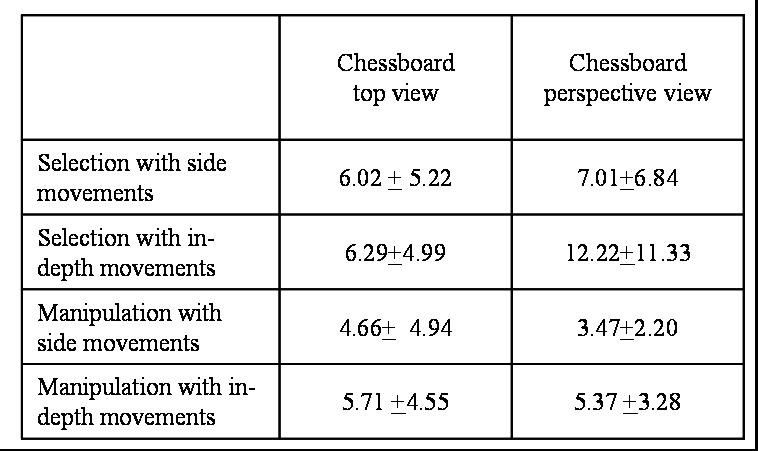
\includegraphics[width=.7\textwidth]{table.jpg}
\end{table}

\begin{table}[]
\centering
\caption{My caption}
\label{my-label}
\begin{tabular}{lllll}
teste & teste & teste & teste & teste \\
a     & b     & c     & d     & e     \\
f     & g     & h     & i     &       \\
      &       &       &       &
\end{tabular}
\end{table}

\section{References}
\bibliographystyle{sbc}
\bibliography{sbc-template}

\end{document}

